\documentclass[12pt,letterpaper]{article}          % Single-sided printing for the library
%\documentclass[12pt,twoside]{article}             % Double-sided printing

%Start Package declarations
%==========================================================================%
%Graphics
\usepackage{graphics}
\usepackage{graphicx}
\usepackage{svg}
\usepackage{tikz}
\usetikzlibrary{shapes,arrows,positioning}
\usepackage{blox}
\usepackage{pgfgantt} %For making the gantt chart
\usepackage{lscape}
%--------------------------------------------------------------------------%
%Formatting
\usepackage{bold-extra}
\usepackage{setspace}
\usepackage{hanging} %hanging indents for bib
\usepackage{microtype}  %micro typographic extensions, for bib(?)
                        %^ pkg. somehow got rid of bib hyphenation issues?!?
\usepackage{tabularx}
\usepackage{array}
\renewcommand\arraystretch{1.2}
\usepackage[autostyle=true,english=american]{csquotes} %Formatting for quotation marks
\MakeOuterQuote{"}
\usepackage{float}
\usepackage{subcaption}
%--------------------------------------------------------------------------%
%Maths
\usepackage{amsmath}
\usepackage{amssymb}
%--------------------------------------------------------------------------%
%Utilities
% \usepackage{showframe}
\usepackage{layout}
\usepackage[
    backend=biber,
    style=ieee,
    sorting=none,
    isbn=false,
    url=false
]{biblatex}
\AtEveryBibitem{
    \clearfield{note}
}
\addbibresource{6_references/references.bib}
\usepackage{hyperref}
\hypersetup{breaklinks=true,colorlinks=true,linkcolor=blue,urlcolor=magenta,citecolor=cyan} %Hyperref links settings
\usepackage{lipsum} %Filler words
\usepackage{comment}
\usepackage{calc} %mix and match units
\usepackage[english]{babel}  %language support
\usepackage{comment}    %block comments!
%==========================================================================%
%End Package declarations

\def\authorName{Nashr El Auliya}
\def\thesisName{3-Dimensional Model-Based Dynamic Feedback Control for Soft Robots}
\newcommand{\imgcite}[1]{Image taken from \cite{#1}.}
\def\sectionautorefname{Section}
\def\subsectionautorefname{Sub-section}

\begin{document}
%==========================================================================%
% This file contains all the necessary setup and commands to create
% the preliminary pages according to the buthesis.sty option.

\title{A BU Thesis Latex Template}

\author{Joe Candidate}

% Type of document prepared for this degree:
%   1 = Master of Science thesis,
%   2 = Doctor of Philosophy dissertation.
\degree=2

\prevdegrees{B.S., Some University, 2016\\
	M.S., Another University, 2018}

\department{Department of Electrical and Computer Engineering}

% Degree year is the year the diploma is expected, and defense year is
% the year the dissertation is written up and defended. Often, these
% will be the same, except for January graduation, when your defense
% will be in the fall of year X, and your graduation will be in
% January of year X+1
\defenseyear{2024}
\degreeyear{2024}

% For each reader, specify appropriate label {First, Second, Third},
% then name, and title. IMPORTANT: The title should be:
%   "Professor of Electrical and Computer Engineering",
% or similar, but it MUST NOT be:
%   Professor, Department of Electrical and Computer Engineering"
% or you will be asked to reprint and get new signatures.
% Warning: If you have more than five readers you are out of luck,
% because it will overflow to a new page. You may try to put part of
% the title in with the name.
\reader{First}{First M. Last, PhD}{Professor of Electrical and Computer Engineering}
\reader{Second}{First M. Last}{Associate Professor of \ldots}
\reader{Third}{First M. Last}{Assistant Professor of \ldots}

% The Major Professor is the same as the first reader, but must be
% specified again for the abstract page. Up to 4 Major Professors
% (advisors) can be defined. 
\numadvisors=2
\majorprof{First M. Last, PhD}{{Professor of Electrical and Computer Engineering\\Secondary appointment}}
\majorprofb{First M. Last, PhD}{{Professor of Computer Science}}
%\majorprofc{First M. Last, PhD}{{Professor of Astronomy}}
%\majorprofd{First M. Last, PhD}{{Professor of Biomedical Engineering}}

%%%%%%%%%%%%%%%%%%%%%%%%%%%%%%%%%%%%%%%%%%%%%%%%%%%%%%%%%%%%%%%%  

%                       PRELIMINARY PAGES
% According to the BU guide the preliminary pages consist of:
% title, copyright (optional), approval,  acknowledgments (opt.),
% abstract, preface (opt.), Table of contents, List of tables (if
% any), List of illustrations (if any). The \tableofcontents,
% \listoffigures, and \listoftables commands can be used in the
% appropriate places. For other things like preface, do it manually
% with something like \newpage\section*{Preface}.

% This is an additional page to print a boxed-in title, author name and
% degree statement so that they are visible through the opening in BU
% covers used for reports. This makes a nicely bound copy. Uncomment only
% if you are printing a hardcopy for such covers. Leave commented out
% when producing PDF for library submission.
%\buecethesistitleboxpage

% Make the titlepage based on the above information.  If you need
% something special and can't use the standard form, you can specify
% the exact text of the titlepage yourself.  Put it in a titlepage
% environment and leave blank lines where you want vertical space.
% The spaces will be adjusted to fill the entire page.
\maketitle
\cleardoublepage

% The copyright page is blank except for the notice at the bottom. You
% must provide your name in capitals.
\copyrightpage
\cleardoublepage

% Now include the approval page based on the readers information
% Once the approval page is approved by the Mugar Library staff, please
% comment out the "\approvalpagewithcomment" line and uncomment "\approvalpage"
\approvalpagewithcomment
%\approvalpage
\cleardoublepage

% Here goes your favorite quote. This page is optional.
\newpage
%\thispagestyle{empty}
\phantom{.}
\vspace{4in}

\begin{singlespace}
\begin{quote}
  \textit{Facilis descensus Averni;}\\
  \textit{Noctes atque dies patet atri janua Ditis;}\\*
  \textit{Sed revocare gradum, superasque evadere ad auras,}\\
  \textit{Hoc opus, hic labor est.}\hfill{Virgil (from Don's thesis!)}
\end{quote}
\end{singlespace}

% \vspace{0.7in}
%
% \noindent
% [The descent to Avernus is easy; the gate of Pluto stands open night
% and day; but to retrace one's steps and return to the upper air, that
% is the toil, that the difficulty.]

\cleardoublepage

% The acknowledgment page should go here. Use something like
% \newpage\section*{Acknowledgments} followed by your text.
\newpage
\section*{\centerline{Acknowledgments}}
Here go all your acknowledgments. You know, your advisor, funding agency, lab
mates, etc., and of course your family.

As for me, I would like to thank Jonathan Polimeni for cleaning up old LaTeX
style files and templates so that Engineering students would not have to suffer
typesetting dissertations in MS Word. Also, I would like to thank IDS/ISS
group (ECE) and CV/CNS lab graduates for their contributions and tweaks to this
scheme over the years (after many frustrations when preparing their final
document for BU library). In particular, I would like to thank Limor Martin who
has helped with the transition to PDF-only dissertation format (no more printing
hardcopies -- hooray !!!)

The stylistic and aesthetic conventions implemented in this LaTeX
thesis/dissertation format would not have been possible without the help from
Brendan McDermot of Mugar library and Martha Wellman of CAS.

Finally, credit is due to Stephen Gildea for the MIT style file off which this
current version is based, and Paolo Gaudiano for porting the MIT style to one
compatible with BU requirements.

\vskip 1in

\noindent
Janusz Konrad\\
Professor\\
ECE Department
\cleardoublepage

% The abstractpage environment sets up everything on the page except
% the text itself.  The title and other header material are put at the
% top of the page, and the supervisors are listed at the bottom.  A
% new page is begun both before and after.  Of course, an abstract may
% be more than one page itself.  If you need more control over the
% format of the page, you can use the abstract environment, which puts
% the word "Abstract" at the beginning and single spaces its text.

\begin{abstractpage}
% ABSTRACT

Have you ever wondered why this is called an \emph{abstract}? Weird thing is
that its legal to cite the abstract of a dissertation alone, apart from the
rest of the manuscript.

\end{abstractpage}
\cleardoublepage

% Now you can include a preface. Again, use something like
% \newpage\section*{Preface} followed by your text

% Table of contents comes after preface
\tableofcontents
\cleardoublepage

% If you do not have tables, comment out the following lines
\newpage
\listoftables
\cleardoublepage

% If you have figures, uncomment the following line
\newpage
\listoffigures
\cleardoublepage

% List of Abbrevs is NOT optional (Martha Wellman likes all abbrevs listed)
\chapter*{List of Abbreviations}

{\color{red} As per BU library instructions, the list of abbreviations must be in alphabetical order by the {\bf abbreviation}, not by the explanation, or it will be returned to you for re-ordering. {\bf This comment must be removed in the final document.}}

\begin{center}
  \begin{tabular}{lll}
    \hspace*{2em} & \hspace*{1in} & \hspace*{4.5in} \\
    CAD  & \dotfill & Computer-Aided Design \\
    CO   & \dotfill & Cytochrome Oxidase \\
    DOG  & \dotfill & Difference Of Gaussian (distributions) \\
    FWHM & \dotfill & Full-Width at Half Maximum \\
    LGN  & \dotfill & Lateral Geniculate Nucleus \\
    ODC  & \dotfill & Ocular Dominance Column \\
    PDF  & \dotfill & Probability Distribution Function \\
    $\mathbb{R}^{2}$  & \dotfill & the Real plane \\
  \end{tabular}
\end{center}
\cleardoublepage

% END OF THE PRELIMINARY PAGES

\newpage
\endofprelim


\section{Abstract} \label{abstractsec}
%----------| comments & notes |----------%
% 1> other past work in 3D soft robot control exists. 
% 2> want to distinguish ours versus others. That's where your literature review comes in! 
% 3> working on model based control, which can be used to (eventually) certify safety unlike learned controllers
% 4> manipulator is under large gravitational loads that could violate modeling assumptions 
% 5> hardware focused rather than simulation. Let me know what else you find as you dig through other prior work

%----------| abstract outline |----------%
%----------| 1. Big problem statement about subject of study (1 stnc.)
The physical characteristics of soft robots inherently promise an ability to perform complex motions, as well as to safely and compliantly interact with sensitive environments. 
%----------| 2. Crucial part of story, not met yet and serves as limitation (1 stnc.)
While trajectory tracking and environmental interaction control strategies for planar motion have been developed along with motion plans for it, it has yet to be robustly translated to three dimensions. 
%----------| 3. "Article addresses limitation by [research insight here]" (1 stnc.)
This proposed thesis thus aims to develop a three-dimensional, model-based, closed loop dynamic controller for continuous soft robots.
%----------| 4. Technical specifics of problem + solution to them and eng. reasons/motivations (1-2 stnc.)
%In the interest of leveraging the "physical guarantees" afforded to us by a dynamic model to eventually allow for safety certification, the controller that this work aims to develop shall be a model-based one.
To develop a robust formulation of this controller, gravitational loads that could potentially violate model assumptions must be dynamically accounted for. Kinematic singularities inherent to the dynamic model used must also be analytically or numerically managed.
%----------| 5. Research approach and experiments to be done (2-3 stnc.)
A suitable dynamic model to underpin the control system must first either be formulated, augmented from an existing one, or selected. Then the model must be validated either analytically or simulatively, before the control system can subsequently be built around it. The controller may then finally be validated through hardware implementation.
%----------| 6. Future directions to address THIS work's limitations OR statement referring back to start (1 stnc.)
%Probably won't need this part
%\cleardoublepage

\section{Topic Background} \label{backgroundsec}
%---------| background outline |---------%
%---------| 1. Define what model-based controls is
\subsection{Model-based Controls in Soft Robotics}
Much of controls theory as a field has progressed in parallel to the advances in our understanding of dynamic modeling. In fact, much of the advancements in controls theory were driven by the need to supplement the gaps in our dynamic models. Starting from the frequency domain and linear controllers, to nonlinear controllers, and most recently machine learning. 

The implementation of control strategies for standard rigid robots has followed this line of progression. Algorithms built around the dynamical model of the robot itself came first, then only recently did strategies employing machine learning began to be implemented--mostly to handle unpredictable scenarios beyond the models' assumptions. Control strategies of the former kind are known as \textit{model}-based controls, where controllers are designed based on models that mathematically represent the robot's dynamics \cite{rakhmatillaev_integrative_2025}. It should be apparent that this has been the case since the dynamics of a rigid-bodied robot can more readily be modelled. 

On the other hand, the development of control strategies for \textit{soft} robots have followed the opposite direction: much of the early works in soft robotics controls employed machine learning strategies due to the high level of complexity and dimensionality required in the dynamical models. Thus, \textit{learning}-based controls were the model for soft robot control strategies through the formative years of the field. Only in recent years did this precedent began to be re-assessed, particularly with the advent of \textit{finite}-dimensional modelling (FDM) techniques compatible with the continuum dynamics of soft robots \cite{della_santina_model-based_2023}.
%----------------------------------------%     
%---------| 2. Model-based vs, learning-based; 
\subsection{Model- vs. Learning-based Controls}
Model- and learning-based controls differ in the fundamental methodology that underpin \textit{how} each approach steers their dynamic systems. Consider some steady-state open-loop dynamic system expressed in state space as $\mathbf{\dot{x}}=\mathbf{f}(\mathbf{x})$, the application of a model- and learning-based controller--respectively--to the system may be represented according to \autoref{modelvslearn}.

\def\sysDyTerms{
    \underline{\dot{q}}=\mathbf{f}(\underline{q},\underline{u})
}

\begin{table}[!ht]
    \centering
    \begin{tabularx}{0.9\textwidth}{|*{2}{>{\centering\arraybackslash}X|}}
        \hline
        Model-based & Learning-based \\
        \hline
        \raggedright Given \par 
        \centering\arraybackslash $\begin{aligned}
            \sysDyTerms & \xrightarrow[\text{for}]{\text{solve}} \underline{u}(\underline{q},\underline{\bar{q}},...)\\
            \mathbf{f}(\underline{q},\underline{u}) & \rightarrow \mathbf{f}(\underline{q},\underline{u}(\underline{q},\underline{\bar{q}}))
        \end{aligned}$ \par
        \raggedright Such that \par 
        \centering\arraybackslash $\underline{\dot{q}} \approx \underline{\bar{\dot{q}}}$ \par & 
        \raggedright Given some dataset \par 
        \centering\arraybackslash 
            $X = \{(\underline{q_0},\underline{u_0}),\dots,(\underline{q_i},\underline{u_i})\}$ \par
        $\begin{aligned}
            X & \xrightarrow[\text{from}]{\text{extract}} \underline{u}^{\text{learned}}
        \end{aligned}$ \par
        \raggedright Such that \par
        \centering\arraybackslash
            $\underline{\dot{q}} \approx \underline{\bar{\dot{q}}}$ \\
        \hline
    \end{tabularx}
    \caption{High-level generalization of model- vs. learning-based controllers, where $\underline{\bar{\dot{q}}}$, $\underline{\bar{q}}$ describes the desired/reference configuration.}
    \label{modelvslearn}
\end{table}

% \raggedright\arraybackslash Where $\underline{\bar{\dot{q}}}$, $\underline{\bar{q}}$ describes the desired/reference configuration

The distinction between model- and learning-based control approaches may be described using the functional framework presented above. In both approaches, some input $\mathbf{u}$ is now introduced to the previously steady-state system. The system becomes \textit{closed}-loop when a controller that uses the system output to determine the control input is implemented (see \autoref{openvsclosed}). %<-- need diagram to help explain!
In this scenario, $f(\mathbf{x,e,t,...})$ can be considered the controller. It functionally relates the system output/current state--and typically error $\mathbf{e}$ and time as well--to the control input. 

\begin{figure}[h!]
    \centering
    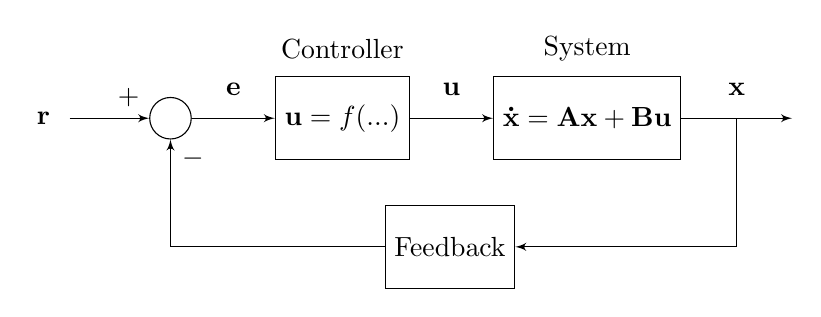
\begin{tikzpicture}
        \bXInput[$\mathbf{r}$]{a}
        \bXComp*{b}{a}{}{-}{+}{}
        \bXLink{a}{b}
        \bXBlocL[3]{c}{
            $\mathbf{u}=f(...)$        
        }{b}
        \bXLinkName[0.7]{b-c}{$\mathbf{e}$}
        \bXLinkName[2.5]{c}{Controller}
        \bXBlocL[3]{d}{
            $\mathbf{\dot{x}=Ax + Bu}$
        }{c}
        \bXLinkName[0.7]{c-d}{$\mathbf{u}$}
        \bXLinkName[2.5]{d}{System}
        \bXOutput[4]{e}{d}
        \bXLink{d}{e}
        \bXLinkName[0.7]{d-e}{$\mathbf{x}$}
        \bXBranchy{d-e}{f}
        \bXBlocr[8]{g}{Feedback}{f}
        \bXLinkyx{d-e}{g}
        \bXLinkxy{g}{b}
    \end{tikzpicture}
    \caption{A generic closed-loop system, the control input is a function of desired state $\mathbf{r}$ and output $\mathbf{x}$.}
    \label{openvsclosed}
\end{figure}


For model-based controls, designing the controller based on the dynamics of the systems means tuning $\mathbf{u}$ to the $\mathbf{A}$ and $\mathbf{B}$ matrices. A conveniently acceptable way of interpreting $\mathbf{\bar{f}}$ is to regard $\mathbf{A}$ as the system's steady-state behavior, and $\mathbf{B}$ as the system's response to control inputs. The two matrices \textit{must} sufficiently describe the system dynamics before $\mathbf{u}$ can be designed to steer the system towards the desired configuration. Formulating $\mathbf{A}$, $\mathbf{B}$, and $\mathbf{u}$ while respecting their inter-dependency thus becomes inherent to the model-based approach.
  
Formulating models that allow the input to be solved in a mathematically managable way, while simultaneously remaining faithfully representative of the \textit{actual} system behavior becomes one of model-based controls' biggest challenges. Learning-based controls circumvent this by using data-driven techniques and learning algorithms to arrive at $\mathbf{u}$. In some cases, $\mathbf{\bar{f}}$ may even be left unknown and the full system is wholly formulated by the learning medium ($\mathbf{g(x,u)}$ in \autoref{modelvslearn}).

\begin{comment} 
    Learning-based controllers have been known to achieve higher levels of performance with respect to more complex actions, typically at the cost of computational efficiency and/or formal guarantees of safety for the robot's behavior \cite{brunke_safe_2022}. Since the formulation of $\mathbf{g(x,u)}$ and $u_{\text{learned}}$ is handled by the learning medium, we are left without the ability to extract detailed functional information regarding either of them. 
\end{comment}
\begin{table}[h!]
    \centering
    \begin{tabularx}{\textwidth}{
        >{\hsize=0.2\hsize\centering\arraybackslash}X|
        >{\hsize=0.4\hsize\centering\arraybackslash}X|
        >{\hsize=0.4\hsize\centering\arraybackslash}X
        }
        Analysis        & Model-Based & Learning-Based\\ \hline\hline
        \raggedleft Advantages      & 
        Meaningful information regarding the dynamics and inputs of the system are preserved &
        Known to achieve higher maneuvering performance and better robustness\newline
        \cite{rakhmatillaev_integrative_2025}\\ \hline
        \raggedleft Disadvantages   &
        Less robust and adaptable at handling system configurations in fringe scenarios\newline
        \cite{rakhmatillaev_integrative_2025}, \cite{brunke_safe_2022} &
        More complex and typically lacks formal guarantees of safety\newline
        \cite{brunke_safe_2022}\\
    \end{tabularx}
    \caption{An assessment of Model- and Learning-Based controls.}
    \label{comparison}
\end{table}

A general assessment of the benefits and drawbacks between the two approaches is presented in \autoref{comparison}. While both approaches bring different things to the table--and extensive research continue to be conducted on both, the author has decided to explore the model-based approach for this proposed thesis.
%----------------------------------------%  
%---------| 3. Brief overview/lit. review of contemporary models
\subsection{Some "Control-Oriented" Models}
It was mentioned earlier that in the formulation of the dynamical model to develop a controller around, towing the balance between mathematical simplicity and physical accuracy is one of the major challenges in model-based controls. While this continues to be true, continuum dynamics-compatible FDM techniques has also indeed broken considerable ground with regards to this issue. In their exact formulation, the dynamics of a soft robot is effectively an infinite-dimensional system. Such a system cannot be described without the use of partial differential equations (PDEs). However, by applying the appropriate assumptions, approximations, and/or discretization to the dynamical model of the soft robot, the system's description may be reliably "minimized" into a \textit{finite}-dimensional system that can be described with ordinary differential equations (ODEs) instead.

One of the most widely-implemented family of FDM techniques is the Piecewise Constant Strain (PCS) approximations (see \autoref{rodandpcs}). It is a family of discretization methods applied to a type of approximation for soft robot dynamics known as "rod models". It is extremely common for soft robots to be "thin" and/or "elongated": to have one physical dimension dominate the other two. In that regard, such soft robots may be approximated as a rod with the continuum mechanics of one too--hence rod models. At the heart of this methodology is the assumption that volumetric deformations may be neglected, and modeling the dynamics around the dominant central axis is sufficient \cite{della_santina_model-based_2023}.

\begin{figure}[h!]
    \centering
    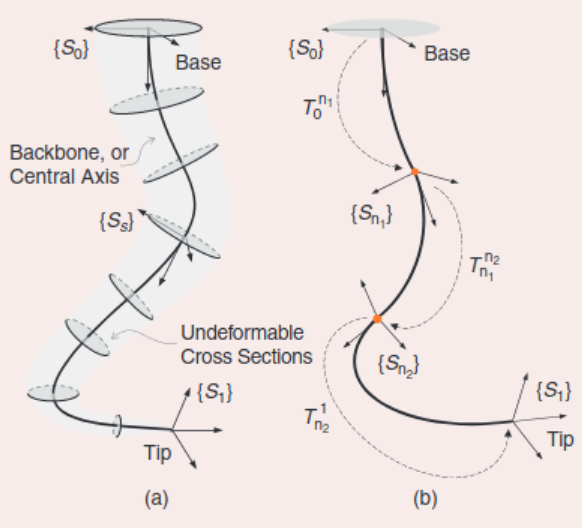
\includegraphics[width=0.4\textwidth]{graphics/rodandpcs.png}
    \caption{a) "Elongated" soft robots as described in rod models. b) PCS discretization applied to the rod model. Image taken from Della Santina et al. \cite{della_santina_model-based_2023}.}
    \label{rodandpcs}
\end{figure}

Among the many implementations of PCS, the planar Piecewise Constant Curvature (PCC) model has been extensively used in soft robotics throughout the last decade. Its approximation of the robot as pieces of constant-curvature arcs linked together in series with mutually tangent connection points makes the kinematics and Jacobian formulation for the model \textit{closed}-form \cite{websteriii_design_2010}. A dynamic feedback controller using this model was developed in \cite{della_santina_model-based_2020}, with an implementation of a trajectory generator for the controller formulated in \cite{dickson_real-time_2025}. 

There are many viable models out there that can be used as the basis for the controller that this proposed thesis seeks to develop, a selection of them that seems promising with respect to the scope of this proposed thesis will be outlined in this proposal.
%\cleardoublepage

\section{Prior Work} \label{priorsec}
%Include prior work here (i.e. Juan and Akua's)
%\cleardoublepage

\section{Research Approach} \label{approachsec}
Research approach

\section{Proposed Timeline} \label{timelinesec}
%Include timeline for completion, along with proposed semester(s) and credits
Research Approach 1: Dec 2025\\
Research Approach 2: Jan 2025\\
Research Approach 3: Mar 2025\\
aaaa\\
aaaa\\
aaaa
\cleardoublepage

\section{References}
\nocite{*}
\printbibliography[heading=none]
%Add references/bibliography

%==========================================================================%
\end{document}